\documentclass{article}
\setlength{\parskip}{5pt} % esp. entre parrafos
\setlength{\parindent}{0pt} % esp. al inicio de un parrafo
\usepackage{amsmath} % mates
\usepackage[sort&compress,numbers]{natbib} % referencias
\usepackage{url} % que las URLs se vean lindos
\usepackage[top=25mm,left=20mm,right=20mm,bottom=25mm]{geometry} % margenes
\usepackage{hyperref} % ligas de URLs
\usepackage{graphicx} % poner figuras
\usepackage[spanish]{babel} % otros idiomas
\usepackage[utf8]{inputenc}
\author{Karla Ocañas \\ Gabryiel Bailon \\ Miguel Rodrigo \\ Alfredo Llanes \\ Betsaida Ruedas} % author
\title{Tarea 2} % titulo
\date{\today}

\begin{document} % inicia contenido

\maketitle % cabecera

\section{Introducci\'{o}n}\label{intro} % seccion y etiqueta
Desde el punto de vista fisiológico, la mano representa la extremidad efectora del miembro superior. Sin embargo, esta no es sólo un órgano de ejecución, es también un receptor sensorial extremadamente sensible y preciso cuya información es indispensable para retroalimentar su propia acción.\\
\\
La mano del hombre es una excelente herramienta, capaz de ejecutar innumerables acciones gracias a su función esencial: la prensión. Está dotada de una gran riqueza funcional que le procura una abundancia de posibilidades en las posiciones, los movimientos y las acciones.\\
\\
Las amputaciones de miembro superior se producen por enfermedades, traumas de toda índole, y por el conflicto armado. Dentro de los traumas, se encuentran accidentes de tránsito, violencia común, accidentes laborales, enfrentamientos armados y minas antipersonales. El 40 porciento de las lesiones de la mano producidas por accidentes laborales o de trabajo, comprometen en mayor porcentaje los dedos índice y pulgar.



\section{Desarrollo}

{Biomecánica de la mano.} \\
\\
La construcción de prótesis de la mano se ha estudiado y desarrollado desde hace siglos atrás, pero n los últimos años con ayuda de de las nuevas tecnologías se ha logrado grandes avances con técnicas de modelamiento y diseño de mecanismos; acompañado de la gran variedad de materiales, control automático y artificial que realizan la integración con la interfaz hombre-maquina que permiten el desarrollo y la obtención de prótesis que no solo simulen el funcionamiento de los movimientos, si no también que garanticen una estética adecuada para el usuario \\
\\
\\
Cuando los pacientes presentan amputación a nivel de la muñeca, requiere el uso de una prótesis para esto existe dos posibilidades: la primera es utilizar una prótesis pasiva(cosmética) y la segunda es optar por las activas, estas a su vez se dividen en propulsión asistida (mioeléctrica, eléctrica y neumática y propulsión muscular(mecánicas)\cite{ff2}\textbf .\\
\\
\\
\\
\\
\\
\\

\begin{figure} [htp]% figura
    \centering
    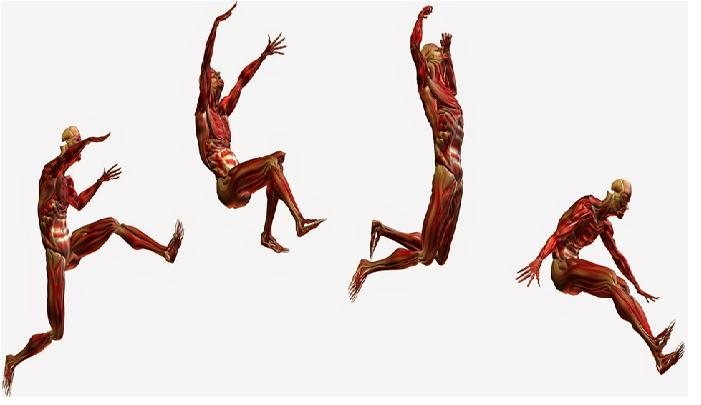
\includegraphics[width=150mm]{biomecanica1.png} % archivo
    \caption{Tipos de protesis}
    \label{grafica}
\end{figure}


 \\
\begin{description}


{Prótesis estéticas} \\

\begin{description}
\item Las prótesis estéticas, conocidas como prótesis pasivas, no tienen movimiento y solo cubren el aspecto estético del miembro amputado, en la fabricación de las mismas se emplean polímeros como PVC rígido, látex flexible o silicona, estos materiales son empleados por ser más livianos y requieren de menos mantenimiento, ya que no disponen de piezas móviles\cite{ff2}\textbf.\\

\begin{figure} [htp]% figura
    \centering
    \includegraphics[width=70mm]{imagen2.jpg} % archivo
    \caption{Prótesis estética}
    \label{grafica}
\end{figure}
\\
\\
\\
\\
\\
\\
\\

{Prótesis mecanicas} \\
\item Las prótesis mecánicas cumplen funciones básicas como la apertura y cerrado de la mano, limitadas al agarre de objetos grandes y movimientos imprecisos, la señal mecánica es obtenida por medio de otro miembro del cuerpo como el codo o hombro, para ello se implementa un arnés colocado en la espalda el cual generará la movilidad de la prótesis a través de una liga\cite{ff2}\textbf.\\

\begin{figure} [htp]% figura
    \centering
    \includegraphics[width=70mm]{imagen3.jpg} % archivo
    \caption{Prótesis mecánicas}
    \label{grafica}
\end{figure}
\\
\\

{Prótesis eléctricas} \\
\item Las prótesis eléctricas se basan en el uso de motores eléctricos, que pueden ser controlados por medio de servo-controles, pulsantes o interruptores, su principal desventaja es su reparación, su alto costo y su exposición a ambientes hostiles, así como también su peso. En la Figura 3 se puede observar una prótesis eléctrica de la compañía Otto Bock que tiene como principal ventaja el agarre de objetos rápidamente y con precisión de forma activa gracias a los sensores en los dedos\cite{ff2}\textbf.\\

\begin{figure} [htp]% figura
    \centering
    \includegraphics[width=70mm]{imagen4.jpg} % archivo
    \caption{Prótesis eléctricas}
    \label{grafica}
\end{figure}

\\
\\

{Prótesis neumáticas} \\
\item Las prótesis neumáticas hacen uso de aire a presión obtenido por medio de un compresor, su ventaja principal es proporcionar una gran fuerza y rapidez de movimientos; sus desventajas principales son los dispositivos que se implementan para su control y funcionamiento ya que son relativamente grandes y su mantenimiento es costoso y dificultoso\cite{ff2}\textbf.\\

\begin{figure} [htp]% figura
    \centering
    \includegraphics[width=50mm]{imagen5.jpg} % archivo
    \caption{Prótesis neumáticas}
    \label{grafica}
\end{figure}
\\
\\

{Prótesis mioeléctricas} \\
\item Las prótesis mioeléctricas son en la actualidad una de las de mayor aplicación en el mundo, ya que brindan un mayor grado de estética y un elevado porcentaje de precisión y fuerza, basándose en la obtención de señales musculares las mismas que son obtenidas mediante el uso de electrodos que permiten la extracción de la señal que es amplificada, procesada y filtrada al control para el manejo de la prótesis\cite{ff2}\textbf.\\
\\
\begin{figure} [htp]% figura
    \centering
    \includegraphics[width100mm]{imagen6.jpg} % archivo
    \caption{Prótesis mioeléctrica}
    \label{grafica}
\end{figure}

\end{description}

\\
\section{Conclusiones}
La realización de una prótesis de mano conlleva un extenso proceso de investagación acerca del paciente y del tipo de prótesis que vaya a necesitar, como los que se mencionaron anteriormente sease: estéticas, mécanicas, eléctricas, neumáticas o en todo caso mioeléctricas. El conocer todo estos tipos de prótesis existentes crean un amplio espectro en el cual el medico e ingnierio pueden realizar un trabajo acorde a las necesidades y presupuesto del paciente. 

\\
\bibliography{bib}
\bibliographystyle{plainnat}
\end{document}